The identified photopeaks of $^{137}$Cs and $^{241}$Am are depicted in Figure \ref{fig:Peaks}.

\begin{figure}[H]
\centering
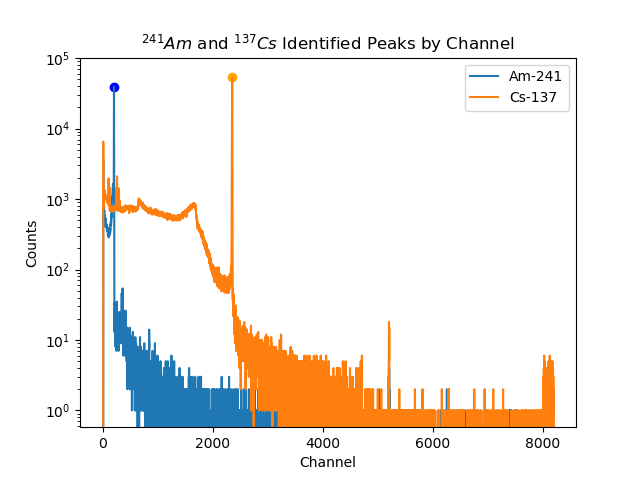
\includegraphics[scale=0.8]{images/Peaks.png}
\caption{Photopeaks of $^{137}$Cs and $^{241}$Am}
\label{fig:Peaks}
\end{figure}

\begin{table}[H]
\centering
\caption{Comparison of Photopeaks for $^{133}$Ba}
\label{tab:Comp}
\begin{tabular}{@{}ll@{}}
Expected (keV) & Calibrated (keV) \\ \midrule
80.9979 & 80.86477260018648 \\
276.3989 & 276.426213420317 \\
302.8508 & 302.8003532152844 \\
356.0129 & 356.10978471575044 \\
383.8485 & 383.8868042870459
\end{tabular}
\end{table}
